\section{Independent Random weight: $\alpha^{i,j}\sim \mathcal{B}(p)$}
Let us consider the case where connections are i.i.d $\sim \mathcal{B}(p)$. The first purpose is to conjecture what is the limit equation for the network. By some heuristic calculation, we expect to see the term:
\[p\cdot \beta\cdot \mathbb{E}[{M_t}]\]
because for $N\rightarrow \infty$, the neurons become asymptotically independent; this means that, applying a law of large numbers,
\[\frac{1}{N}\mathbb{E}\left[\int_0^t\sum_j\sum_k\beta\alpha^{i,j}\delta(s-\tau^j_k)ds\right]=\frac{1}{N} \mathbb{E}\left[\sum_j\sum_k\beta\alpha^{i,j}\mathbb{I}_{\tau^j_k\leq t}\right]=p\cdot \beta\cdot \mathbb{E}[{M_t}]. \] 
So, as a limit equation for the network, we expect the following:
\[X_t=X_0+\int_0^t b(X_s)ds+\beta\cdot p\cdot\mathbb{E}[M_t]+\sigma W_t-M_t\]
with $M_t=\sum_{k\leq 1}\mathbb{I}_{[0,t]}(\tau_k)$.
To justify more rigorously the conjectured equation, we propose the following argument based on a simple model for propagation of chaos. 
\subsection{Derivation of the limit equation in the simpler model}
Propagation of chaos is the phenomenon where some interacting particles become independent at the limit for the number of particles going to infinity. \\
To get an idea of the behaviour of particles in neuronal networks, we consider the simpler model
\begin{equation} \label{SDE} dX^i_t = \frac{1}{N} \sum_{i = 1}^N \alpha^{i, j} X^j_t \ dt + dW^i_t, \end{equation} where $(\alpha^{i, j})_{i, j = 1, ..., N}$ is a family of i.i.d. random variables with finite first momentum and $(W^i)_i$ is a family of independent standard Brownian motions. The family of the r.v.(s) $\alpha^{i, j}$ and that of the Brownian motions $W^i$ are assumed to be independent. \\

We use the technique of \textbf{coupling}. That is, we want to show convergence of (\ref{SDE}) to \begin{equation} \label{bar} d \bar{X}_t = \mathbbm{E} \big[ \alpha \big] \mathbbm{E} \big[ \bar{X}_t \big] dt + d W_t, \end{equation} where $\alpha$ is another r.v. independent of all the $\alpha^{i, j}$ and of Brownian motions and where $W$ is another Brownian motion, with the same independence assumptions. To prove the convergence stated above, let's also introduce the SDE \begin{equation} \label{bar_i} d \bar{X}^i_t = \mathbbm{E} \big[ \alpha \big] \mathbbm{E} \big[ \bar{X}^i_t \big] dt + d W^i_t \end{equation} and let's follow the strategy consisting in proving some kind of "closeness" of (\ref{bar}) with (\ref{bar_i}) and of (\ref{bar_i}) with (\ref{SDE}). That's what we mean by coupling. \\
Our "closeness" concept will be "in law" and, at this point, we can already state that $\bar{X}$ e $\bar{X}^i$ have the same law: we therefore just need to consider $X^i$ and $\bar{X}^i$. \\

We now observe that all the processes $\bar{X}$ and $(\bar{X}^i)_i$ are independent of all the $(\alpha^{i,j})_{i,j}$. \\
We also know that \[ \begin{aligned} d \left( X^i_t - \bar{X}^i_t \right) &= \left( \frac{1}{N} \sum_{j = 1}^N \alpha^{i, j} X^j_t - \mathbbm{E} \big[ \alpha \bar{X}^i_t \big] \right) dt \\ &= \left[ \left( \frac{1}{N} \sum_{j = 1}^N \alpha^{i, j} X^j_t - \frac{1}{N} \sum_{j = 1}^N \alpha^{i, j} \bar{X}^j_t \right) + \left(\frac{1}{N} \sum_{j = 1}^N \alpha^{i, j} \bar{X}^j_t - \mathbbm{E} \big[ \alpha \bar{X}^i_t \big] \right) \right] dt. \end{aligned} \]

If $\alpha^{i, j}$ are bounded by a constant $C$ (or if $\frac{1}{N} \sum_{j = 1}^N | \alpha^{i,j} | \leq C$, where $C$ is a random variable not depending on $i$ nor on $N$), then \[ \left| X^i_t - \bar{X}^i_t \right| \leq \int_0^t \frac{C}{N} \sum_{j = 1}^N \left| X^j_s - \bar{X}^j_s \right| ds + \int_0^t \left| \frac{1}{N} \sum_{j = 1}^N \alpha^{i, j} \bar{X}^j_s - \mathbbm{E} \big[ \alpha \bar{X}^i_s \big] \right| ds. \] By summing over $i$ and dividing by $N$, also defining $\delta_t$ to be the function $\frac{1}{N} \sum_i \left| X^i_t - \bar{X}^i_t \right|$, we get \[ \delta_t \leq C \int_0^t \delta_s ds + \frac{1}{N^2} \int_0^t \sum_{i = 1}^N \left| \sum_{j = 1}^N \left( \alpha^{i, j} \bar{X}^j_s - \mathbbm{E} \big[ \alpha \bar{X}^i_s \big] \right) \right| ds. \]
By using Gronwall's lemma, we then deduce that \[ \delta_t \leq \frac{\exp(C t)}{N^2} \int_0^t \sum_{i = 1}^N \left| \sum_{j = 1}^N \left( \alpha^{i, j} \bar{X}^j_s - \mathbbm{E} \big[ \alpha \bar{X}^i_s \big] \right) \right| ds. \]
Taking the expectation and using the Cauchy-Schwarz inequality, we have the following: \[ \mathbbm{E} [\delta_t] \leq \frac{ \left( \mathbbm{E} \left[ \exp(2 C t) \right] \right)^{1/2}}{N} \int_0^t \sum_{i = 1}^N \left( \frac{1}{N^2} \mathbbm{E} \left[ \left( \sum_{j = 1}^N \left( \alpha^{i, j} \bar{X}^j_s - \mathbbm{E} \big[ \alpha \bar{X}^i_s \big] \right) \right)^2 \right] \right)^{1/2} ds. \]
It is therefore useful to investigate the second moment of $\left( \alpha^{i, j} \bar{X}^j_s - \mathbbm{E} \big[ \alpha \bar{X}^i_s \big] \right)$, which is a finite value $C_2$ \todo{1} \textbf{(EXERCISE)}. Hence: \[ \mathbbm{E} [ \delta_t ] \leq \frac{ \left( \mathbbm{E} \left[ \exp(2 C t) \right] \right)^{1/2}}{N} \int_0^t \sum_{i = 1}^N \left( \frac{1}{N^2} 4 N C_2 \right)^{1/2} ds \leq \frac{\left( \mathbbm{E} \left[ \exp(2 C t) \right] \right)^{1/2} 2 C_2^{1/2} t}{N^{1/2}} . \]

\textbf{NB} It holds that \[ \delta_t \geq W_1 \left( \frac{1}{N} \sum_{i = 1}^N \delta_{X^i_t}, \frac{1}{N} \sum_{i = 1}^N \delta_{\bar{X}^i_t} \right), \] where $W_1(\cdot, \cdot)$ is the $1$-Wasserstein distance. We have therefore proved that the Wasserstein distance goes to $0$, since $\delta_t$ does. \\

\begin{center}
------------------------------------------------------------------------------------------------------------------ \\
\end{center}

\subsection{Blow-up Argument}
We will here present a probabilistic argument for the blow-up, based on the proof presented by Carrilo, Perthame et al. in \cite{caceres_analysis_2010}\todo{verificare la bibliografia}
\begin{theorem}
Assume that drift coefficient satisfies
\[b(v) \geq -\lambda v, \quad \text{for all $-\infty<v\leq1$.}\]
If the initial condition is concentrated around the threshold $1$, there is no global in time solution of the SDE
\[dX_t = b(X_t)dt + \beta\cdot p\cdot e'(t) dt + dW_t - d M_t, \qquad t\geq 0,\]
with a deterministic initial condition $X(0) = x_0 < 1$, with $\beta \in \mathbb{R}^+$.
\end{theorem}
\begin{proof}
The idea is to retrace the proof of Carrillo, Perthame et al.\\
The object of our study is $\mathbb{E}[\varphi_\mu(X_t)]$ with $\varphi_\mu(x)=\exp(\mu x)$. \\
Remember that
\[X_t = X_0 + \int_0^t \Big( b(X_s) + \beta\cdot p e'(s) \Big) ds + W_t - M_t\]
with $M_t=\int_0^t\int_{\mathbb{R}_+}g(X_{s-},z)N(ds,dz)$.
Now we apply the Ito-formula to $\varphi_\mu(X_t)$ (for simplicity, I will omitt $\mu$ in the computation)
\begin{multline*}
\varphi(X_t)=\varphi(X_0)+\int_0^t\underbrace{\varphi'(X_s)}_{\mu\varphi(X_s)} \Big( b(X_s) + \alpha\cdot p e'(s) \Big) ds+\int_0^t \underbrace{\varphi'(X_s)}_{\mu \varphi(X_s)}dW_s+\frac{1}{2}\int_0^t \underbrace{\varphi''(X_s)}_{\mu^2 \varphi(X_s)} ds+\\
\int_0^t \int_{\mathbb{R_+}}\underbrace{[\varphi(X_{s-}+g(X_{s-},z))-\varphi(X_{s-})]}_{\big( \varphi(0)-\varphi(1) \big) \mathbbm{1}_{ \left\{ X_s\leq 1 \right\} }}N(ds,dz).\\
\end{multline*}
Taking the expectation:
\begin{multline*}
\mathbb{E}\left[\varphi(X_t)\right]=\mathbb{E}\left[\varphi(X_0)\right]+\mu\int_0^t\mathbb{E}\left[\varphi(X_s) \Big( b(X_s) + \beta\cdot p e'(s) \Big)\right]ds+\frac{\mu^2}{2}\int_0^t \mathbb{E}\left[\varphi(X_s)\right] ds+\\
\Big(\varphi(0)-\varphi(1)\Big)e(t).\\
\end{multline*}
Defining $F_\mu(t):=\mathbb{E}[\varphi(X_t)]$, we can rewrite the above expression as:
\begin{multline*}
F_\mu(t)=F_\mu(0)+\mu\int_0^t\mathbb{E}\left[\varphi(X_s) \Big( b(X_s) + \beta\cdot p e'(s) \Big) \right]ds+\frac{\mu^2}{2}\int_0^t F_\mu(s)ds+\\
\Big(\varphi(0)-\varphi(1)\Big)e(t).\\
\end{multline*}
Then, using the hypotesis on $b$, we get that
\begin{multline*}
F_\mu(t)\geq F_\mu(0)+\mu\int_0^t\mathbb{E}\left[\varphi(X_s) (\beta \cdot p e'(s)-\lambda X_s )\right]ds+\frac{\mu^2}{2}\int_0^t F_\mu(s)ds+\Big(\varphi(0)-\varphi(1)\Big)e(t) \nonumber\\
\geq F_\mu(0)+\mu\int_0^t(\beta \cdot p e'(s)-\lambda )F_\mu(s)ds+\frac{\mu^2}{2}\int_0^t F_\mu(s)ds+\Big(\varphi(0)-\varphi(1)\Big)e(t),
\end{multline*} that is 
\begin{equation} \label{eq_ret_1} F_\mu(t) \geq F_\mu(0)+\int_0^t\mu\left(\beta\cdot p e'(s)-\lambda+\frac{\mu}{2}\right)F_\mu(s)ds+\Big(\varphi(0)-\varphi(1)\Big)e(t). \end{equation}
Define $\tilde{\lambda}$ as
\[\tilde{\lambda} := \frac{\varphi(1)-\varphi(0)}{\mu\beta p} \]
and let's choose $\mu$ such that
\[-\lambda+\frac{\mu}{2}>0.\]
We can now proceed by stating that:
\begin{multline*}
F_\mu(t) \geq  F_\mu(0) + \int_0^t \mu \beta e'(s)F_\mu(s)ds-\tilde{\lambda}\beta\mu e(t)\\
\geq F_\mu(0)+\int_0^t\mu\beta e'(s)[F_\mu(s)-\tilde{\lambda}]ds.\\
\end{multline*}
In differential form:
\begin{equation}
\frac{d}{dt}F_\mu(t)\geq \mu\beta e'(t)\Big[F_\mu(t)-\tilde{\lambda}\Big].
\end{equation}
\textbf{Claim:} If $F_\mu(0)\geq \tilde{\lambda}$, then $F_\mu(t)\geq \tilde{\lambda}$. \\
This simply comes from an application of Gronwall Lemma to the function $\tilde{F}_\mu(t) := \tilde{\lambda} - F_\mu(t)$. \\

Coming back to (\ref{eq_ret_1}) we get that
\begin{multline*}
F_\mu(t)\geq F_\mu(0)+\int_0^t\mu\left(\beta e'(s)-\lambda +\frac{\mu}{2}\right)F_\mu(s)ds+\tilde{\lambda}\beta\mu e(t)\\
\geq F_\mu(0)+\int_0^t\mu\beta e'(s)F_\mu(s)ds+\int_0^t \mu \left(-\lambda +\frac{\mu}{2} \right) F_\mu(s)ds-\tilde{\lambda}\beta\mu e(t)\\
=F_\mu(0)+\tilde{\lambda}\beta\mu e(t)+\int_0^t \mu \left(-\lambda +\frac{\mu}{2} \right) F_\mu(s)ds-\tilde{\lambda}\beta\mu e(t)\\
=F_\mu(0)+\int_0^t \mu \left( -\lambda +\frac{\mu}{2} \right) F_\mu(s)ds.\\
\end{multline*}
In differential form:
\[ \frac{d}{dt}F_\mu(t) \geq \mu \left( -\lambda+\frac{\mu}{2} \right) F_\mu(t), \]
which implies that:
\begin{equation} \label{contr1} F_\mu(t)\geq \exp \left( \mu \Big( -\lambda+\frac{\mu}{2}t \Big) \right) F_\mu(0). \end{equation}
But we know that
\begin{equation} \label{contr2} F_\mu(t)\leq\exp \big( \mu \big). \end{equation}
From (\ref{contr1}) and (\ref{contr2}) we get a contradiction.
\end{proof}
\begin{remark}\label{rem: bu1}
In summary, fixed an $(\alpha,p)$ the phenomena of blow up holds for initial condition that are concentrated around the threshold, namely for initial condition such that
\[\exists \mu>2\lambda\text{ such that }F_\mu(0)\geq \tilde{\lambda}\text{ with }\tilde{\lambda}=\frac{\phi(1)-\phi(0)}{\mu\beta p} \]
Assuming for simplicity that the initial condition is deterministic, we get:
\[F_\mu(0)=\exp(\mu x_0)\]
So, given a deterministic initial condition, we look for all $p$ such that:
\[p\geq \inf_{\mu\geq 2\lambda}\frac{e^\mu-1}{\mu\alpha e^{\mu x_0}}:=p^+_c(x_0)\]

\todo{commentare il plot?}
\begin{figure}
\centering
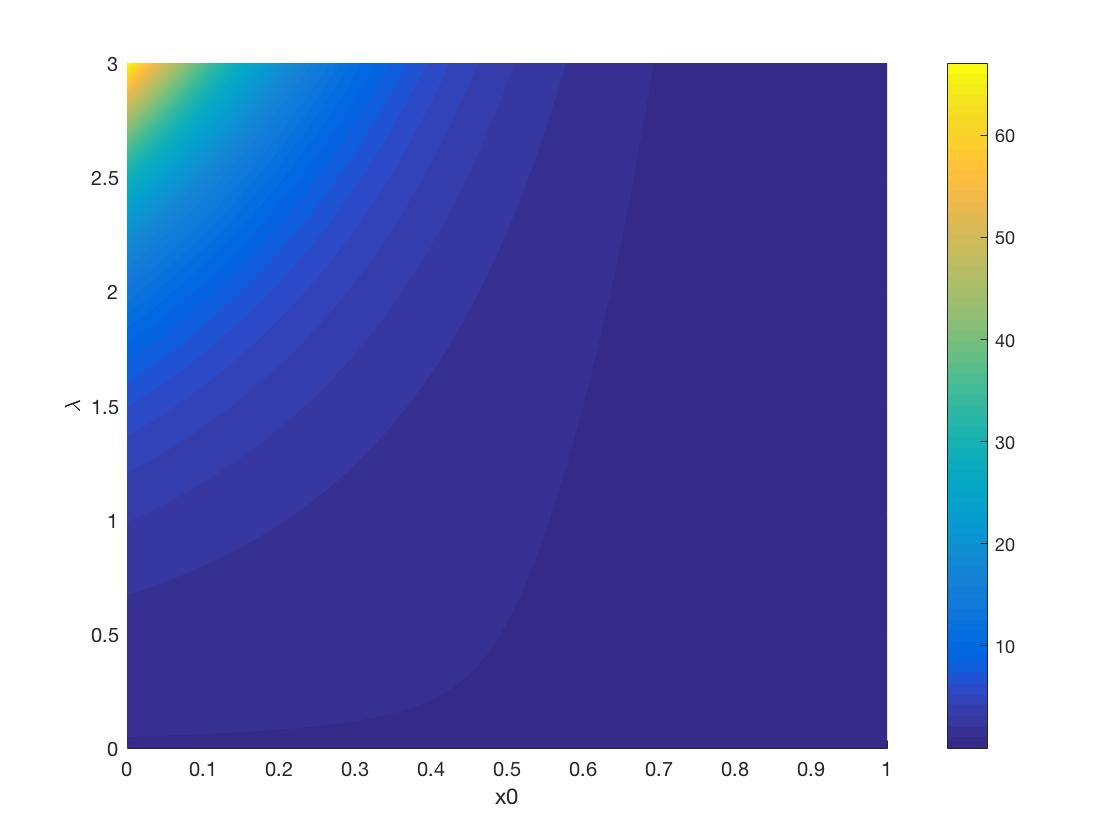
\includegraphics[width=12.5cm]{Upper_bound}
\caption{Plot of the upper bound estimate $p^+_c$ for the threshold $p_c$}
\end{figure}\label{fig:1}
In figure \ref{fig:1} we present the upper bound for the threshold $p^+_c$, varying on the parameter of the drift $\lambda$ and the initial condition $x_0$.
\end{remark}

\subsection{Blow up discussion for the Brownian case}
Let's focus on a particular case, in absence of drift, so $\lambda=0$, with deterministic initial condition $x_0=0.8$ and $\beta=1$. From the previous remark, we get that $p^+_c\sim 0.539$. Moreover by Theorem 5.2 we get that $p^-_c\sim 0.1$.
Through simulations, we look for the critical threshold $p_c(x_0)$ $[p^-_c(x_0),p^+_c(x_0)]$, observing that the threshold is around $0.34$. (In red the result obtained by numerics)\\ 


\begin{tikzpicture}
\draw  (0,0)  (14,1);
\draw[-,thick] (3,0.5)-- (11,0.5);
\draw[-,red] (6.7,0.4)--(6.7,0.6);
\draw[-,red] (7,0.4)--(7,0.6);
\node[red] at (6.7,0.9) {0.38};
\node[red] at (7.15,0.2) {0.39};
\filldraw (3,0.5) circle (1.5pt);
\node at (3,0.9) {$0$};
\node at (4.3,0.9) {$0.1$};
\filldraw (4.3,0.5) circle (1.5pt);
\filldraw (11,0.5) circle (1.5pt);
\filldraw (9,0.5) circle (1.5pt);
\node at (9,0.9) {$0.539$};
\node at (11,0.9) {$1$};
\node[red]  at (5.5,0.1) {G};
\node at (3.5,0.1) {G};
\node[red] at (8.3,0.1) {B-U};
\node at (10,0.1) {B-U};
\end{tikzpicture}

In the more general case, where $\alpha\neq 1$, we get that the threshold for $p$ is simply rescaled by the factor $\alpha$.

\section{Dependent Random Weights}
In this section, we will present a short analysis on the behaviour of the network of neurons, when the connections are dependent. In particular, we will focus on two different kind of interactions, due to random connections.
First, we will focus on the case when $\alpha^i \alpha^j$, where $(\alpha^i)_{i = 1, ..., N}$ are independent Bernoullian r.v.(s) with the same distribution, then :
\begin{equation}
 X^i_t = X^i_0 + \int_0^t b(X^i_s) ds + \frac{\alpha^i}{N} \sum_{j = 1}^N \alpha^{j} M^j_t - M^i_t + W^i_t. \quad  i=1,\cdots,N\label{eq:aiaj}
 \end{equation}
 
Our first purpose is to find out the limit equation. We conjecture that the limit equation for this system is the following:
\begin{equation} \label{eq1} X_t = X_0 + \int_0^t b(X_s) ds + \alpha \mathbbm{E}[\alpha M_t] - M_t + W_t, \end{equation} where $\alpha$ is another Bernoullian r.v. with the same distribution as all the $\alpha^{i}$; or if the limit equation takes the form 

\begin{equation} \label{eq2} X_t = X_0 + \int_0^t b(X_s) ds + \alpha \mathbbm{E}[\alpha] \mathbbm{E}[M_t] - M_t + W_t. 
\end{equation}
with the same hypothesis on $\alpha$.Our guess is that the limit equation is (\ref{eq1}), because of the fact that the processes $X^i$ and $M^i$ should not become independent of $\alpha^i$, even if the network size tends to infinity. So, we shouldn't be able to observe the term $\mathbbm{E}[\alpha]\mathbbm{E}[M_t]$, but we should see a term like $\mathbbm{E}[\alpha M_t]$ instead. \\

Moreover, heuristically, the system (\ref{eq:aiaj}) define a a network that consist of two different component: the first is a complete sub-network, composed by neurons all connected beetwen themselves, so neurons of the subnetwork feel all the neurons of the subnetwork. The second component is  made of isolated neurons. So we expect at the limit equation for average behaviour a randomness, to catch out the duality of the population and moreover we expect that the weight of the kick is calibrated by size of the subnetwork:

\[ \alpha \mathbbm{E} \Big[ \alpha M_t \Big], \]

The equation (\ref{eq2}) can describe the limit equation for a newtwork of neurons, that still present two different population: one of isolated neurons and the other of neurons that interact with all the other neurons, with probability $p$. So with interaction term:

\begin{eqnarray*}
\frac{\alpha^i}{N} \sum_{j = 1}^N \alpha^j M^j_t
\end{eqnarray*}

Numerically, if the limit equation were (\ref{eq2}), then the interaction term $\frac{\alpha^i}{N} \sum_{j = 1}^N \alpha^j M^j_t$ should behave, for $N$ large enough, like $\frac{\alpha^i \cdot p}{N} \sum_{j = 1}^N M^j_t$. We therefore compare numerically those two terms. 

\begin{center}
  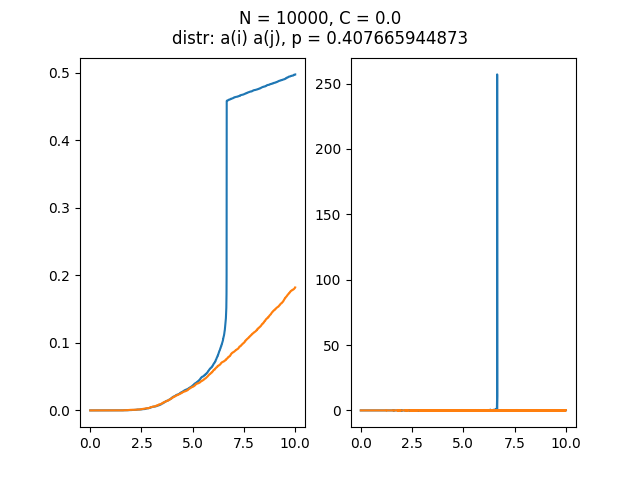
\includegraphics[scale=0.8]{confronto_indip_1.png}\\
  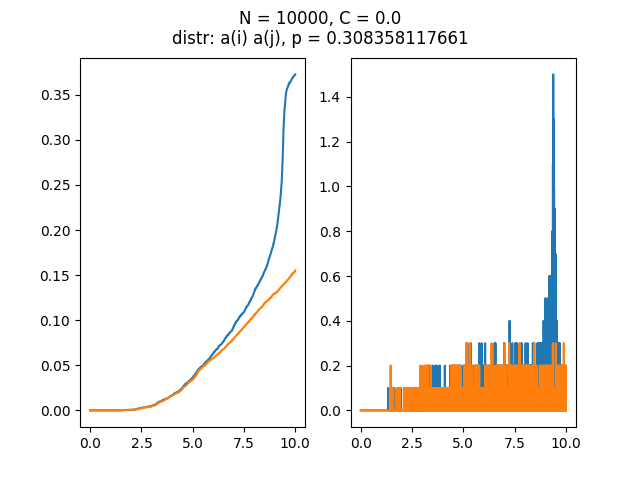
\includegraphics[scale=0.8]{confronto_indip_7.png}\\
  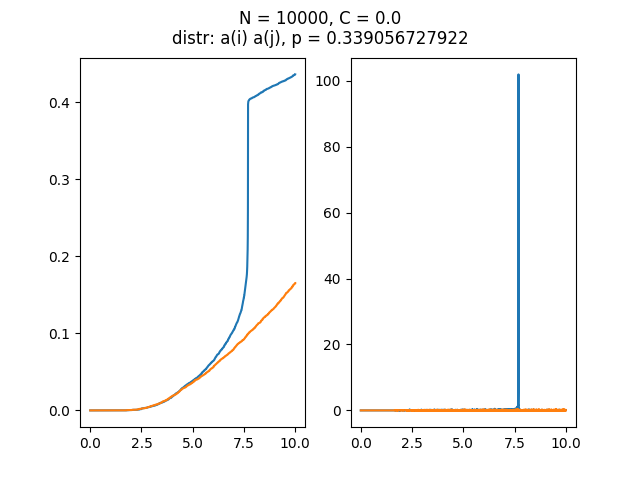
\includegraphics[scale=0.8]{confronto_indip_8.png}\\
  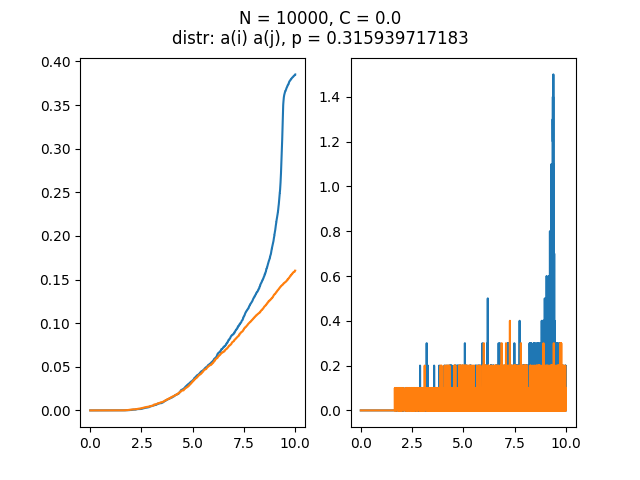
\includegraphics[scale=0.8]{confronto_indip_10.png}\\
\end{center}

We observe a quite different behaviour. \todo{Explain data} \\

\begin{remark}
Remembering the natural splitting of the network explained just above, we get that, considering the limit of (\ref{eq1}) \[ \alpha \mathbbm{E} \big[ \alpha M_t \big] = \alpha \mathbbm{E} \left[ M_t \cdot \mathbbm{1}_{ \left\{ \alpha = 1 \right\} } \right] = \alpha p \cdot \mathbbm{E} \big[ M_t \left| \ \alpha = 1 \right. \big]. \] Regarding the limit form of (\ref{eq2}): 

\begin{equation} \label{limit2} 
\begin{aligned} \alpha p \cdot \mathbbm{E} \big[ M_t \big] &= \alpha p \Big( \mathbbm{E} \left[ M_t \left| \mathbbm{1}_{ \left\{ \alpha = 1 \right\} } \right. \right] \cdot p  + \mathbbm{E} \left[ M_t \left| \mathbbm{1}_{ \left\{ \alpha = 0 \right\} } \right. \right] \cdot (1 - p) \Big) \\ & = \alpha p^2 \cdot \mathbbm{E} \Big[ M_t \left| \ \alpha = 1 \right. \Big] + \alpha p (1 - p) \cdot \mathbbm{E} \Big[ M_t \left| \ \alpha = 0 \right. \Big] 
\end{aligned} 
\end{equation}

\textbf{CLAIM:} the leading term for blow up in (\ref{limit2}) is 
\[ \alpha p^2 \cdot \mathbbm{E} \Big[ M_t \left| \ \alpha = 1 \right. \Big], \] 
So we can expect that the threshold for blow up for (\ref{eq1}), $p^2_c\approx \sqrt{p^1_c}$
%so that, at the limit, we expect that the bahaviour of (\ref{2}) is the same as that of (\ref{1}), except for the additional multiplicative constant $p$. \todo{adattare la dim. del blow-up a questo caso} \todo{Verificare che $\alpha p$ è critico per il primo caso e  $\sim \alpha p^2$ lo è per il secondo caso} \\
\end{remark}
\subsection{Derivation of the limit equation in the simpler model for $\alpha_{i,j}=\alpha_i\alpha_j$}
We now study the limit behaviour of \[ X^i_t = X^i_0 + \int_0^t b(X^i_s) ds + \frac{\alpha^i}{N} \sum_{j = 1}^N \alpha^j M^j_t - M^i_t + W^i_t \] (where $\alpha^i$ are i.i.d. Bernoullian) from a theoretical point of view. Particularly, we consider the simpler model already introduced before, thet is the one described by \[ d X^i_t = \frac{\alpha^i}{N} \sum_{j = 1}^N \alpha^j X^j_t dt + d W^i_t. \]
We also introduce, following the notation already used, the processes $\bar{X}^i$ described by \[ d \bar{X}^i_t = \alpha^i \mathbbm{E} \left[ \alpha^i \bar{X}^i_t \right] dt + d W^i_t. \]
Assuming that $X^i$ and $\bar{X}^i$ have the same initial conditions, we get \[ X^i_t - \bar{X}^i_t = \int_0^t \frac{\alpha^i}{N} \sum_{j = 1}^N \alpha^j \Big( X^j_s - \bar{X}^j_s \Big) ds + \int_0^t \left( \frac{\alpha^i}{N} \sum_{j = 1}^N \alpha^j \bar{X}^j_s - \alpha^i \mathbbm{E} \left[ \alpha^i \bar{X}^i_s \right] \right) ds. \]
Multiplying by $\alpha^i$, summing over $i$ and dividing by $N$, we can assert that \begin{multline*} \frac{1}{N} \sum_{i = 1}^N \alpha^i \Big| X^i_t - \bar{X}^i_t \Big| \leq \int_0^t \left( \frac{1}{N} \sum_{i = 1}^N (\alpha^i)^2 \right) \left( \frac{1}{N} \sum_{i = 1}^N \alpha^i \Big| X^i_s - \bar{X}^i_s \Big| \right) ds + \\ + \int_0^t \left( \frac{1}{N} \sum_{i = 1}^N (\alpha^i)^2 \right) \left| \frac{1}{N} \sum_{j = 1}^N \alpha^j \bar{X}^j_s - \mathbbm{E} \left[ \alpha^i \bar{X}^i_s \right] \right| ds. \end{multline*}
Defining $\tilde{\delta}_t = \frac{1}{N} \sum_{i = 1}^N \alpha^i \big| X^i_t - \bar{X}^i_t \big|$, we can write that \[ \tilde{\delta}_t \leq \left( \frac{1}{N} \sum_{i = 1}^N (\alpha^i)^2 \right) \left[ \int_0^t \tilde{\delta}_s ds + \int_0^t \left| \frac{1}{N} \sum_{j = 1}^N \alpha^j \bar{X}^j_s - \mathbbm{E} \left[ \alpha^i \bar{X}^i_s \right] \right| ds \right]. \]
By using Gronwall's lemma: \[ \tilde{\delta_t} \leq \left( \frac{1}{N} \sum_{i = 1}^N (\alpha^i)^2 \right) \exp \left( \frac{1}{N} \sum_{i = 1}^N (\alpha^i)^2 t \right) \int_0^t \left| \frac{1}{N} \sum_{j = 1}^N \alpha^j \bar{X}^j_s - \mathbbm{E} \left[ \alpha^i \bar{X}^i_s \right] \right| ds. \]
Also defining $\delta_t = \mathbbm{E}[\tilde{\delta_t}]$, $A = \left( \frac{1}{N} \sum_{i = 1}^N (\alpha^i)^2 \right)$, taking the expectation and using the Cauchy-Schwarz inequality, we have \[ \delta_t \leq \Big( \mathbbm{E} \left[ A^2 \exp \big( 2 A t \big) \right] \Big)^{1/2} \int_0^t \left( \mathbbm{E} \left[ \left( \frac{1}{N} \sum_{j = 1}^N \alpha^j \bar{X}^j_s - \mathbbm{E} \left[ \alpha^i \bar{X}^i_s \right] \right)^2 \right] \right)^{1/2} ds. \]
We can manage the last term in the expression above as we did before. In fact: \[ \mathbbm{E} \left[ \left( \frac{1}{N} \sum_{j = 1}^N \alpha^j \bar{X}^j_s - \mathbbm{E} \left[ \alpha^i \bar{X}^i_s \right] \right)^2 \right] = \mathbbm{E} \left[ \left( \frac{1}{N} \sum_{j=1}^N \alpha^j \bar{X}^j_s \right)^2 \right] - \Big( \mathbbm{E} \left[ \alpha^i \bar{X}^i_s \right] \Big)^2. \]
Expanding the first term in the last line above, we then get \begin{multline*} \frac{1}{N^2} \mathbbm{E}\left[ \sum_{j = 1}^N \Big( \alpha^j \bar{X}^j_s \Big)^2 + \sum_{j \neq k} \alpha^j \alpha^k \bar{X}^j_s \bar{X}^k_s \right] - \Big( \mathbbm{E} \left[ \alpha^i \bar{X}^i_s \right] \Big)^2 = \\ = \frac{1}{N} \Big( \mathbbm{E} \left[ \left( \alpha^i \bar{X}^i_s \right)^2 \right] - \left( \mathbbm{E} \left[ \alpha^j \bar{X}^i_s \right] \right)^2 \Big) \end{multline*}
Therefore \[ \delta_t \leq \left( \mathbbm{E} \left[ A^2 \exp \big( 2 A t \big) \right] \right)^{1/2} \cdot \frac{1}{N^{1/2}} \int_0^t \Big( \mathbbm{E} \left[ \left( \alpha^i \bar{X}^i_s \right)^2 \right] - \left( \mathbbm{E} \left[ \alpha^j \bar{X}^i_s \right] \right)^2 \Big)^{1/2} ds. \]

The derivation of equation  (\ref{eq2}) from the network of interacting neurons:
\begin{equation}
 X^i_t = X^i_0 + \int_0^t b(X^i_s) ds + \frac{\alpha^i}{N} \sum_{j = 1}^N \alpha^{j} M^j_t - M^i_t + W^i_t. \quad  i=1,\cdots,N\label{eq:aiaj}
 \end{equation}
adapted to the case of the simple model, follows from a very similar argument.
\todo{argomentare meglio}
\subsection{Blow-up Argument}
\begin{theorem}
Assume that drift coefficient satisfies
\[b(v) \geq -\lambda v, \quad \text{for all $-\infty<v\leq1$.}\]
If the initial condition is concentrated around the threshold $1$, there is no global in time solution of the SDE
\begin{equation} \label{limit1} X_t = X_0 + \int_0^t b(X_s) ds + \alpha p \cdot \mathbbm{E} \left[ M_t \right] + W_t - M_t, \end{equation}
with $\alpha\sim\mathcal{B}(p)$ and deterministic initial condition $X(0) = X_0 < 1$.
\end{theorem}

\begin{proof}
Taking the function $\varphi_{\mu}(x) = \exp ( \mu x )$ for some $\mu > 0$ and using the Ito-formula, we have that \begin{multline*} \varphi_\mu (X_t) = \varphi_\mu (X_0) + \int_0^t \mu \varphi(X_s) \Big( b(X_s) + \alpha p e'(s) + \frac{\mu}{2} \Big) ds + \\ + \int_0^t \mu \varphi(X_s) d W_s + \int_0^t (\varphi(X_{s-} - 1) - \varphi(X_{s-})) dM_s.  \end{multline*}
Particularly, the last term reduces to $\big( \varphi(0) - \varphi(1) \big) \cdot M_t$, which is negative. Multiplying the equation above by $\alpha$, recalling that $b(v) \geq - \lambda v$ by hypotesis and that $X_t \leq 1$, we then get \begin{multline*} \alpha \varphi_\mu (X_t) = \alpha \varphi_\mu (X_0) + \int_0^t \mu \alpha \varphi(X_s) \Big( -\lambda + \alpha p e'(s) + \frac{\mu}{2} \Big) ds + \\ + \int_0^t \mu \alpha \varphi(X_s) d W_s + \big( \varphi(0) - \varphi(1) \big) \cdot \alpha M_t. \end{multline*}
The stochastic integral above remains a martingale, even after multiplying by $\alpha$, which implies that, taking the expectation and calling $F^\alpha_\mu(t) := \mathbbm{E} \Big[ \alpha \varphi_\mu (X_t) \Big]$: \[ F^\alpha_\mu(t) = F^\alpha_\mu(0) + \int_0^t \mathbbm{E} \left[ \mu \alpha \varphi(X_s) \Big( -\lambda + \alpha p e'(s) + \frac{\mu}{2} \Big) \right] ds + \Big( \varphi(0) - \varphi(1) \Big) \mathbbm{E}[\alpha M_t]. \] The random variable $\alpha \in \big\{ 0, 1 \big\}$ and $M_t$ is non-negative, which makes it possible to state that $\mathbbm{E} \big[ \alpha M_t \big] \leq \mathbbm{E} \big[ M_t \big]$. Therefore, since $\big( \varphi(0) - \varphi(1) \big)$ is negative, 
\begin{equation} 
\label{starting} F^\alpha_\mu(t) \geq F^\alpha_\mu(0) + \int_0^t \mu \left( - \lambda + \frac{\mu}{2} \right) F^\alpha_\mu(s) ds + \int_0^t \mu p e'(s) F^\alpha_\mu(s) ds + \Big( \varphi(0) - \varphi(1) \Big) e(t). \end{equation}
We now assume that \[ - \lambda + \frac{\mu}{2} > 0, \] so that \[ F^\alpha_\mu(t) \geq F^\alpha_\mu(0) + \int_0^t \mu p e'(s) F^\alpha_\mu(s) ds + \Big( \varphi(0) - \varphi(1) \Big) e(t); \] calling $\tilde{\lambda} := \frac{1}{\mu p} \big( - \varphi(0) + \varphi(1) \big)$, we end up with \[ F^\alpha_\mu(t) \geq F^\alpha_\mu(0) + \int_0^t \mu p e'(s) \Big( F^\alpha_\mu(s) - \tilde{\lambda} \Big) ds. \] Hence, if $F^\alpha_\mu(0) \geq \tilde{\lambda}$, then \[ F^\alpha_\mu(t) \geq \tilde{\lambda}. \] Starting again from (\ref{starting}): \[ F^\alpha_\mu(t) \geq F^\alpha_\mu(0) + \int_0^t \mu \left( -\lambda + \frac{\mu}{2} \right) F^\alpha_\mu(s) ds, \] which implies that \[ F^\alpha_\mu(t) \geq F^\alpha_\mu(0) \exp \left( \mu \Big( - \lambda + \frac{\mu}{2} \Big) t \right). \] This is a contradiction because $X_t \leq 1$ and $\alpha \in \{ 0, 1 \}$, which means that \[ F^\alpha_\mu (t) \leq e^\mu. \]
\end{proof}

\begin{remark}
As explained in Remark \ref{rem: bu1}, ther is blow-up when
\[\exists \mu>2\lambda\text{ such that }F_\mu(0)\geq \tilde{\lambda}\text{ with }\tilde{\lambda}=\frac{\phi(1)-\phi(0)}{\mu p} \]
Assuming for simplicity that the initial condition is deterministic, we get:
\[F^\alpha_\mu(0)=p\cdot\exp(\mu x_0)\]
So, given a deterministic initial condition, we look for all $p$ such that:
\[p\geq \sqrt{\inf_{\mu\geq 2\lambda}\frac{e^\mu-1}{\mu\alpha e^{\mu x_0}}}:=p^{+,1}_c(x_0)\]

In figure \ref{fig:2} we present the upper bound for the threshold $p^{+,1}_c$, varying on the parameter of the drift $\lambda$ and the initial condition $x_0$.

\begin{figure}\label{fig:2}
\centering
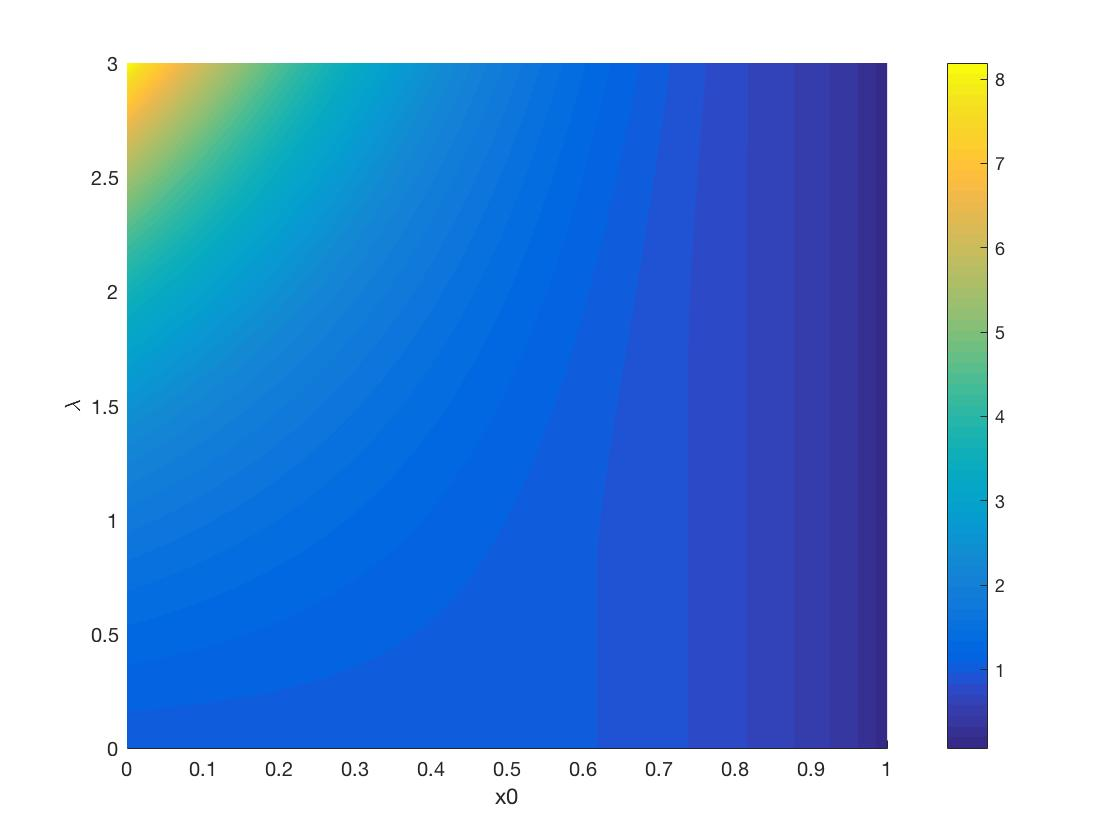
\includegraphics[width=12.5cm]{Upper_bound2}
\caption{Plot of the upper bound estimate $p^{+,1}_c$ for the threshold $p_c$}
\end{figure}
\end{remark}


\begin{theorem}
Assume that drift coefficient satisfies
\[b(v) \geq -\lambda v, \quad \text{for all $-\infty<v\leq1$.}\]
If the initial condition is concentrated around the threshold $1$, there is no global in time solution of the SDE
\begin{equation} \label{limit1} X_t = X_0 + \int_0^t b(X_s) ds + \alpha  \cdot \mathbbm{E} \left[ \alpha M_t \right] + W_t - M_t, \end{equation}
with a deterministic initial condition $X(0) = x_0 < 1$ and $\alpha\sim\mathcal{B}(p)$.
\end{theorem}
\begin{proof}
The strategy is almost the same of the previous case, namely the main object of the proof is 
$F^\alpha_\mu(t) := \mathbbm{E} \Big[ \alpha \varphi_\mu (X_t) \Big]$. The identity satisfied by $F^\alpha_\mu$ obtained using Ito Formula:

\[ F^\alpha_\mu(t) = F^\alpha_\mu(0) + \int_0^t \mathbbm{E} \left[ \mu \alpha \varphi(X_s) \Big( -\lambda + \alpha e_\alpha'(s) + \frac{\mu}{2} \Big) \right] ds + \Big( \varphi(0) - \varphi(1) \Big) \mathbbm{E}[\alpha M_t]. \]
with $e_\alpha(t)=\mathbb{E}[\alpha M_t]$. With the same calculation of the previous case, we get
\begin{equation*} 
\label{starting} F^\alpha_\mu(t) \geq F^\alpha_\mu(0) + \int_0^t \mu \left( - \lambda + \frac{\mu}{2} \right) F^\alpha_\mu(s) ds + \int_0^t \mu e'_\alpha(s) F^\alpha_\mu(s) ds + \Big( \varphi(0) - \varphi(1) \Big) e_\alpha(t).
 \end{equation*}
 The only difference with respect to the previous case is that in the calculation we have $e_\alpha(t)$ instead of $e(t)$.
\end{proof}
\begin{remark}
As before, there is blow-up when
\[\exists \mu>2\lambda\text{ such that }F^\alpha_\mu(0)\geq \tilde{\lambda}\text{ with }\tilde{\lambda}=\frac{\phi(1)-\phi(0)}{\mu } \]
Assuming for simplicity that the initial condition is deterministic, we get:
\[F_\mu(0)=p\cdot\exp(\mu x_0)\]
So, given a deterministic initial condition, we look for all $p$ such that:
\[p\geq \inf_{\mu\geq 2\lambda}\frac{e^\mu-1}{\mu e^{\mu x_0}}:=p^{+,2}_c(x_0)\]

So the upper bound varying on the parameters $(x_0,\lambda)$ is the same of figure \ref{fig:1}.
\end{remark}

\subsection{Blow up discussion for the Brownian case}
Let's focus on the case where the network include a non complete subnetwork  (\ref{eq2}) , in absence of drift, so $\lambda=0$, with deterministic initial condition $x_0=0.8$. From the previous remark, we get that $p^+_c\sim 0.7201$. Through simulations, we look for the threshold value $p_c$.\\

\begin{tikzpicture}
\draw  (0,0)  (14,1);
\draw[-,thick] (3,0.5)-- (11,0.5);
\draw[-] (7,0.4)--(7,0.6);
\node[red] at (7,0.9) {0.53};
\filldraw (3,0.5) circle (1.5pt);
\node at (3,0.9) {$0$};
\filldraw (11,0.5) circle (1.5pt);
\filldraw (9,0.5) circle (1.5pt);
\node at (9,0.9) {$0.7201$};
\node at (11,0.9) {$1$};
\node[red] at (4.5,0.1) {G};
\node[red] at (8,0.1) {B-U};
\node at (10,0.1) {B-U};
\end{tikzpicture}
\todo{fare simulazioni accurate in $[0.51,0.55]$}
 
Indeed in the case where the network generate a complete subnetwork (\ref{eq1}), we get

\begin{tikzpicture}
\draw  (0,0)  (14,1);
\draw[-,thick] (3,0.5)-- (11,0.5);
\draw[-] (5,0.4)--(5,0.6);
\node[red] at (5,0.9) {0.34};
\filldraw (7,0.5) circle (1.5pt);
\node at (7,0.9) {0.539};
\filldraw (3,0.5) circle (1.5pt);
\node at (3,0.9) {$0$};
\filldraw (11,0.5) circle (1.5pt);
\node at (11,0.9) {$1$};
\node[red] at (4.5,0.1) {G};
\node at (9,0.1) {B-U};
\node[red]  at (6,0.1) {B-U};
\end{tikzpicture}
\todo{fare simulazioni accurate in $[0.3,0.34]$}

\subsection{Comparison between the two models}
We here consider the following SDEs:
\begin{align*}
  X^i_t = X^i_0 + \int_0^t b(X^i_s) ds + \frac{\alpha^i}{N} p \sum_{j = 1}^N M^j_t + W^i_t - M^i_t, \\
  X^i_t = X^i_0 + \int_0^t b(X^i_s) ds + \frac{\alpha^i}{N} \sum_{j = 1}^N \alpha^j M^j_t + W^i_t - M^i_t,
\end{align*}
with the usual definitions. We already know that those SDEs converge respectively, as $N \to +\infty$, to the limit SDEs:
\begin{align*}
  X_t = X_0 + \int_0^t b(X_s) ds + \alpha p \mathbbm{E} \big[ M_t \big] + W_t - M_t, \\
  X_t = X_0 + \int_0^t b(X_s) ds + \alpha \mathbbm{E} \big[ \alpha M_t \big] + W_t - M_t,
\end{align*}
again with the usual definitions.

These last SDEs could easily be rewritten as:
\begin{align*}
  X_t = X_0 + \int_0^t b(X_s) ds + \alpha p \Big( p \cdot \mathbbm{E} \big[ M_t \big| \  \alpha = 1 \big. \big] + (1-p) \cdot \mathbbm{E} \big[ M_t \big| \  \alpha = 0 \big. \big] \Big) + W_t - M_t, \\
  X_t = X_0 + \int_0^t b(X_s) ds + \alpha \Big( p \cdot \mathbbm{E} \big[ M_t \big| \  \alpha = 1 \big. \big] \Big) + W_t - M_t.
\end{align*}

Assuming, as usual, a deterministic initial condition $X_0 = x_0$ and a function $b = 0$, we finally get:
\begin{align}
  X_t = x_0 + \Big( \alpha p^2 \cdot \mathbbm{E} \big[ M_t \big| \  \alpha = 1 \big. \big] + \alpha p (1-p) \cdot \mathbbm{E} \big[ M_t \big| \  \alpha = 0 \big. \big] \Big) + W_t - M_t, \label{eq_1} \\
  X_t = x_0 + \Big( \alpha p \cdot \mathbbm{E} \big[ M_t \big| \  \alpha = 1 \big. \big] \Big) + W_t - M_t. \label{eq_2}
\end{align}

We now study equation (\ref{eq_1}) and compare it to (\ref{eq_2}). First, let us consider the term $\mathbbm{E} \big[ M_t \big| \ \alpha = 0 \big. \big]$: this is the expectation of the process $M_t$ when we assume no interaction. Therefore, we may identify $\mathbbm{E} \big[ M_t \big| \ \alpha = 0 \big. \big]$ with $\mathbbm{E} \big[ \tilde{M}_t \big]$, where $\tilde{M}_t$ solves the SDE: \[ \tilde{X}_t + \tilde{M}_t = x_0 + \tilde{W}_t, \qquad \tilde{M}_t = \left\lfloor \left( \sup_{[0, t]} \big( \tilde{X}_s + \tilde{M}_s \big) \right)_+ \right\rfloor. \] Hence, \[ \tilde{X}_s + \tilde{M}_s = x_0 + \tilde{W}_s, \] which means that \[ \mathbbm{E} \left[ \tilde{M}_t \right] = \mathbbm{E} \left[ \left\lfloor \left( x_0 + \sup_{[0, t]} \tilde{W}_s \big) \right)_+ \right\rfloor \right] . \] Calling $f_t$ the density of the running maximum of Brownian motion until time $t$, we get that \[ \mathbbm{E} \left[ \tilde{M}_t \right] = \int_{\mathbb{R}} \left\lfloor \left( x_0 + x \big) \right)_+ \right\rfloor f_t(x) dx. \]
Recall that $f_t(x) = \sqrt{2/\pi t} \ \exp \big(- x^2 / 2t \big)$, so that the expression above becomes \begin{align*} \mathbbm{E}\left[ \tilde{M}_t \right] &= \sqrt{\frac{2}{\pi t}} \int_{\mathbb{R}} \left\lfloor \left( x_0 + x \big) \right)_+ \right\rfloor \ \exp \left( - \frac{x^2}{2t} \right) dx \\ &= \sqrt{\frac{2}{\pi t}} \int_{-x_0}^{+\infty} \left\lfloor \left( x_0 + x \big) \right)_+ \right\rfloor \ \exp \left( - \frac{x^2}{2t} \right) dx \\ &= \frac{4}{\sqrt{\pi}} \int_{-x_0 / \sqrt{2t}}^{+\infty} \left\lfloor \left( x_0 + \sqrt{2 t} x \big) \right)_+ \right\rfloor \ \exp \left( - x^2 \right) dx \\ &= \frac{4}{\sqrt{\pi}} \sum_{k \in \mathbbm{N}} k \cdot \int_{ (-x_0 + k) / \sqrt{2t}}^{ (-x_0 + k + 1) / \sqrt{2t}} \exp \left( - x^2 \right) dx. \end{align*}

Particularly, calling $e_0(t) := \mathbbm{E}\left[ \tilde{M}_t \right]$, we see that the function $e_0$ is differentiable and its derivative is \[ e_0'(t) = \frac{1}{t} \sqrt{\frac{2}{\pi t}} e^{- \frac{x_0^2}{2t}} \sum_{k \in \mathbbm{N}} k \left[ (-x_0+k) e^{\frac{-k^2+2x_0k}{2t}} - (-x_0+k+1)e^{\frac{-(k+1)^2+2x_0(k+1)}{2t}} \right]. \]

Remembering that $x_0 < 1$, so that $-k^2 + 2x_0 k \geq 0$ whenever $k \geq 2$, we obtain the following: \begin{multline*} e_0'(t) = \frac{1}{t} \sqrt{\frac{2}{\pi t}} e^{- \frac{x_0^2}{2t}} \Bigg[ (1-x_0) \left[ e^{\frac{-1+2x_0}{2t}} - e^{\frac{-2(1-x_0)}{t}} \right] + \\ + \sum_{k \geq 2} k \left[ (-x_0+k) e^{\frac{-k^2+2x_0k}{2t}} - (-x_0+k+1)e^{\frac{-(k+1)^2+2x_0(k+1)}{2t}} \right] \Bigg]; \end{multline*}
also observing that $e^{-1/t}$ is increasing in $t$, we could bound $e_0'(t)$ with: \[ \frac{1}{t} \sqrt{\frac{2}{\pi t}} e^{- \frac{x_0^2}{2t}} \Bigg[ C_{x_0, T} + \sum_{k \geq 2} k \left[ (-x_0+k) e^{\frac{-k^2+2x_0k}{2T}} - (-x_0+k+1)e^{\frac{-(k+1)^2+2x_0(k+1)}{2T}} \right] \Bigg], \] that is, increasing the constant $C_{x_0, T}$ if necessary, \begin{align*} e_0'(t) \leq C_{x_0, T} \frac{1}{t \sqrt{t}} e^{- \frac{x_0^2}{2t}}. \\ \end{align*}

We now come back to (\ref{eq_1}) and (\ref{eq_2}). \\
Particularly, we can rewrite (\ref{eq_1}) in the form: \begin{equation} \label{eq_1_rew} X_t = x_0 + \alpha p (1-p) \int_0^t e_0'(s) ds + \Big( \alpha p^2 \cdot \mathbbm{E} \big[ M_t \big| \  \alpha = 1 \big. \big] \Big) + W_t - M_t. \end{equation}
With respect to (\ref{eq_2}), we observe an additional (random) drift term and an additional multiplicative constant $p$ in the interaction term. \\

\section{Independent Bernoullian R.V.(s) with parameter $p_N$}
Considering the network where the synaptic weights are given by the family of i.i.d. Bernoullian random variables $(\alpha^{i, j})_{i, j} \sim \mathcal{B}(p_N)$, we want to compare numerically the behaviour of the interaction term \begin{equation} \label{4} \frac{c}{N \cdot p_N} \sum_{j=1}^N \alpha^{ij} M^j_t \end{equation} with the interaction term 
\begin{equation} \label{5} \frac{1}{N} \sum_{j = 1}^N \beta^{i, j} M^j_t, \end{equation} now $(\beta^{i, j})_{i, j} \sim \mathcal{B}(c)$ are independent and identically distributed. \\
We observe that (\ref{5}) has the same limit behaviour as \begin{equation} \label{6} \frac{c}{N} \sum_{j = 1}^N M^j_t \end{equation} and, given the computational advantage of using this form, we will compare (\ref{4}) to (\ref{6}). \\

%\textbf{REMARK:} the scaling term in (\ref{4}) is $N \cdot p_N$; ideally, we would take the degree of the node as the scaling term, which is \[ \sum_{j = 1}^N \alpha^{i, j}. \] The expectation of that term is exactly $N p_N$, so that, for computational simplicity, we take $N p_N$ as the scaling term itself.
%\title{Spiking Cascade in a Neuronal Network with Random Synaptic Weights dependent on the number of particles}

We deal with the neuronal network described by the equation \[ X^i_t = X^i_0 + \int_0^t b(X^i_s) ds + \frac{\beta}{p_N \cdot N} \sum_{j = 1}^N \alpha^{i, j}_N M^j_t + W^i_t - M^i_t, \] where $\alpha^{i, j}_N$ are Bernoullian random variables with parameter $p_N$ dependent on $N$, the total number of neurons in the network. We are interested in three cases:
\begin{itemize}
  \item $p_N \cdot N = \log^{1/2}(N)$;
  \item $p_N \cdot N = \log(N)$;
  \item $p_N \cdot N = \log^2(N)$.
\end{itemize}

Particularly, a distinctive characteristic of this network is that it is possible to have a neuron spiking more than once at the same instant of time. \\
This can happen for three reasons. \\
First, it is possible that one neuron receives a cumulative kick by all the other particles which is greater than $1$: so the potential of a neuron can jump from a potential less than $1$ to a potential greater than $2$. We will however ignore this behaviour, considering it as a single spike. \\
Secondly, it is possible that a neuron spikes, that its kick makes other particles spike and that those, in turn, make the first particle spike again. This behaviour may repeat again: when it repeats just for a finite number of times, we call it a \textbf{"finite cascade"}.
The third and last possibility is that the cascading behaviour just described goes on infinitely many times: we call it an \textbf{"infinite cascade"}. This happens when there are some particles spiking which mutually reinforce each other: \todo{FALSE}{\textbf{it can be shown that those particles have to be among those with a degree bigger than $\lceil p_N N / \beta \rceil$ FALSE!!!}}.
Let's give an estimate for the probability of multiple spikes.
We here find an upper bound on the probability that a neuron has degree bigger than $\lceil p_N N / \beta \rceil$. \\
We are therefore interested in computing \[ \mathbbm{P} \left[ \frac{1}{N} \sum_{j = 1}^N \alpha^{1, j}_N \geq \frac{p_N}{\beta} \right], \] where the apex $1$ may be substituted by any other index $i$. \\


Observing that $p_N / N$ is bigger than $p_N$ and using the Cramer's Theorem (in the context of Large Deviation Theory), we find out that 

\begin{equation}\label{upperbound}
\mathbbm{P} \left[ \frac{1}{N} \sum_{j = 1}^N \alpha^{1, j}_N \geq \frac{p_N}{\beta} \right] \leq e^{- N \cdot \Lambda^* \left( \frac{p_N}{N} \right) }, \end{equation}
 where \[ \Lambda^*(x) := x \log \left( \frac{x}{p_N} \right) + (1-x) \log \left( \frac{1 - x}{1 - p_N} \right).\]

 \begin{remark}[Estimate on the upper bound for the probability to have a multiple spikes]
Taking the logarithm and multiplying by $-1$ the term $e^{- N \cdot \Lambda^* \left( \frac{p_N}{N} \right) }$, we have that \begin{equation} \label{other:claim} - \log \left( e^{- N \cdot \Lambda^*\left(\frac{p_N}{\beta}\right)} \right) = \frac{1}{\beta} \log \left( \frac{1}{\beta} \right) \log^k(N) + \left( N - \frac{\log^k(N)}{\beta} \right) \log \left( \frac{\beta N  - \log^k(N)}{\beta N - \beta \log^k(N)} \right). \end{equation} Tha last part above is \begin{multline*} \left( N - \frac{\log^k(N)}{\beta} \right) \log \left( \frac{\beta N  - \log^k(N)}{\beta N - \beta \log^k(N)} \right) = \\ = \left( N - \frac{\log^k(N)}{\beta} \right) \log \left( 1 - \frac{1 - \beta}{\beta} \frac{\log^k(N)}{N - \log^k(N)} \right). \end{multline*}
Therefore, the last expression becomes \[ \left( N - \frac{\log^k(N)}{\beta} \right) \left( - \frac{1 - \beta}{\beta} \frac{\log^k(N)}{N - \log^k(N)} + o \left( \left( \frac{\log^{k}(N)}{N - \log^k(N)} \right)^2 \right) \right), \] which can be rewritten as \begin{multline*} \frac{ \beta N - \log^k(N)}{\beta} \left( - \frac{(1 - \beta) \log^k(N)}{\beta \big( N - \log^k(N) \big) } \right) + \frac{ \beta N - \log^k(N)}{\beta} \cdot o \left( \left( \frac{\log^{k}(N)}{N - \log^k(N)} \right)^2 \right) = \\ = \frac{ \beta N - \log^k(N) }{ \beta N - \beta \log^k(N) } \left( - \frac{(1 - \beta) \log^k(N)}{\beta} \right) + \\ + \frac{ \beta N - \log^k(N)}{ \beta N - \beta \log^k(N) } \cdot \frac{ N - \log^k(N) }{ \log^k(N) } \log^k(N) \cdot o \left( \left( \frac{\log^{k}(N)}{N - \log^k(N)} \right)^2 \right). \end{multline*}
Finally, we can again rewrite the expression above as \[ \left( \frac{ \beta N - \log^k(N) }{ \beta N - \beta \log^k(N) } \right) \left( - \frac{1 - \beta}{\beta} + o \left( \frac{\log^{k}(N)}{N - \log^k(N)} \right) \right) \log^k(N). \]
Now, the first term in the expression above converges to $1$ when $N \to +\infty$; similarly, the "small o" multiplied by $\log^k(N)$ goes to $0$ when $N \to +\infty$; this means that, for every $c < 1$, definitively, \[ \left( \frac{ \beta N - \log^k(N) }{ \beta N - \beta \log^k(N) } \right) \left( - \frac{1 - \beta}{\beta} + o \left( \frac{\log^{k}(N)}{N - \log^k(N)} \right) \right) \log^k(N) \geq -c \left( \frac{1-\beta}{\beta} \right) \log^k(N). \]
  
Coming back to (\ref{other:claim}): \[ - \log \left( e^{- N \cdot \Lambda^*\left(\frac{p_N}{\beta}\right)} \right) \geq \left[ \frac{1}{\beta} \left( \log \left( \frac{1}{\beta} \right) - c \right) + c \right] \log^k(N). \]  Calling $C(\beta) := \frac{1}{\beta} \left( \log \left( \frac{1}{\beta} \right) - c \right) + c$, we deduce that \[ e^{- N \cdot \Lambda^*\left(\frac{p_N}{\beta}\right)} \leq e^{- C(\beta) \log^k(N)}. \]
To conclude, we have found that \[ \mathbbm{P} \left[ \frac{1}{N} \sum_{j = 1}^N \alpha^{1, j}_N \geq \frac{p_N}{\beta} \right] \leq e^{- C(\beta) \log^k(N)}. \]
\end{remark}
\begin{theorem}[Large Deviation Result]
Assuming that $\beta<1$, $p_N=\frac{(\log N)^k}{N}$
\[\lim_{N\rightarrow\infty}a^{-1}_N\log\left(\mathbbm{P} \left[ \frac{1}{N} \sum_{j = 1}^N \alpha^{j}_N \geq \frac{p_N}{\beta} \right]\right)=-C(\beta)\]
with $a_N=N\cdot p_N$ and $C(\beta) := \frac{1}{\beta} \left( \log \left( \frac{1}{\beta} \right) - 1 \right) + 1$
\end{theorem}
\begin{proof}
To prove the large deviation result we need an upper bound estimate and a lower bound estimate. The lower bound estimate is the one given in ($\ref{upperbound}$). \todo{dettagli}
The argument for the lower bound is a very classical one, the main tool is given by Cramer Transformation of random variable. 
\begin{equation*}
\mathbbm{P} \left( \frac{1}{N} \sum_{j = 1}^N \alpha^{j}_N \geq \frac{p_N}{\beta} \right)=\mathbbm{P} \left( \frac{1}{N} \sum_{j = 1}^N \tilde{\alpha}^{j}_N \geq \frac{p_N}{\beta} -x\right)
\end{equation*}
where $\tilde{\alpha}^j_x=\alpha^j-x$. Let's consider a family of random variable $\hat{\alpha}^j$ given by Cramer Transformation, so that their CDF is 
\[\hat{F}(x)=\frac{1}{A_N}\int_{-\infty}^x e^{\tau y} dF(y)\]
with $A_N=\exp(-N\cdot C(\beta)\cdot p_N)$.
First, let us choose $x$ such that $\hat{F}$  is a CDF, so such that
\[  A_N= g(\tau)\]
where $\phi$ is the moment generating function of $\tilde{\alpha}^j_x$:
\[x=-\frac{1}{\tau}\log\left( \frac{e^{-C(\beta)}p_N}{1-p_N+e^\tau p_N}\right)\]
Moreover, we impose that the family $\hat{\alpha}^j$ is centered and with positive variance.
\begin{equation}
\mathbb{E}\left[  \hat{\alpha}_1\right]=\hat{g}'(0)=\frac{1}{A_N} g'(\tau)=0\label{mean}
\end{equation}
where $\hat{g}$ is the moment generating function of $\hat{\alpha}_i$.
So we choose
\[\tau=\log\left(\frac{x\cdot(1-p_N)}{(1-x)p_N}\right)\]
namely, the point at which the minimum for $g$ is reached.
Through this choice of $\tau$ we get that the variance is positive and that it does not depend on $N$.
\begin{equation}
VAR\left[\hat{\alpha}^j\right]=\hat{g}''(0)=\frac{1}{A} g''(0)=\frac{g''(0)}{g(\tau)}=\frac{G_1(x)}{G_2(x)}
\end{equation}\label{variance}
\todo{}
Let us verify that
\begin{equation}
\mathbb{P} \left( \frac{1}{N} \sum_{j = 1}^N \alpha^{j}_N \geq \frac{p_N}{\beta} \right)=(A_N)^N\mathbb{E}\left[\exp(-\tau\cdot \underline{\hat{S}}_N)1_{\underline{\hat{S}}_N\geq N\cdot(\frac{p_N}{\beta}-1)}\right]
\end{equation}
where $\underline{\hat{S}}_N$ states for the empirical average.
\begin{align*}
\mathbb{P} \left( \frac{1}{N} \sum_{j = 1}^N \tilde{\alpha}^{j}_N \geq \frac{p_N}{\beta}-x \right)&=
\mathbb{P} \left(\underline{\tilde{S}}_N \geq N\left(\frac{p_N}{\beta}-x\right) \right)\\
&=\int_{x_1+\cdots+x_N\geq N\left(\frac{p_N}{\beta}-x\right)} dF_1(x_1)\cdot\cdots\cdot dF_N(x_N)\\
&=A^N\int_{x_1+\cdots+x_N\geq N\left(\frac{p_N}{\beta}-x\right)}e^{-\tau (x_1+\cdots x_N)} d\hat{F}_1(x_1)\cdot\cdots\cdot d\hat{F}_N(x_N)\\
& = (A_N)^N\mathbb{E}\left[\exp(-\tau\cdot \underline{\hat{S}}_N)1_{\underline{\hat{S}}_N\geq N\cdot(\frac{p_N}{\beta}-1)}\right]
\end{align*}
Because the variance ($\ref{variance}$) does not depend on N, we can apply the TLC to prove that
\[\liminf_{N\rightarrow \infty}\mathbb{E}\left[\exp(-\tau\cdot \underline{\hat{S}}_N)1_{\underline{\hat{S}}_N\geq N\cdot(\frac{p_N}{\beta}-1)}\right]\geq 0\]\todo{scrivere bene i conti}
So we can conclude
\begin{align*}
&\liminf_{N} a_N^{-1}\log{\mathbb{P} \left( \frac{1}{N} \sum_{j = 1}^N \alpha^{j}_N \geq \frac{p_N}{\beta}\right)}\\
&=\liminf_{N} a_N^{-1}\log{(A_N)^N\mathbb{E}\left[\exp(-\tau\cdot \underline{\hat{S}}_N)1_{\underline{\hat{S}}_N\geq N\cdot(\frac{p_N}{\beta}-1)}\right]}\\
&\geq-C(\beta)
\end{align*}
\end{proof}


\begin{remark}[Probability of having a network with no possible cascade behaviour]

We are here interested in computing \begin{align*} \mathbbm{P} \left[ \exists i \Big| \ \frac{1}{N} \sum_{j = 1}^N \alpha^{i, j}_N \geq \frac{p_N}{\beta} \right] &= 1 - \mathbbm{P} \left[ \forall i, \ \frac{1}{N} \sum_{j = 1}^N \alpha^{i, j}_N < \frac{p_N}{\beta} \right] \\ &= 1 - \left( \mathbbm{P} \left[ \frac{1}{N} \sum_{j = 1}^N \alpha^{1, j}_N < \frac{p_N}{\beta} \right] \right)^N, \end{align*} because of the independence properties on the random connections $\alpha^{i, j}_N$. \\

By using the inequality found in the previous paragraph:
\begin{align*} \mathbbm{P} \left[ \exists i \Big| \ \frac{1}{N} \sum_{j = 1}^N \alpha^{i, j}_N \geq \frac{p_N}{\beta} \right] &= 1 - \left( 1 - \mathbbm{P} \left[ \frac{1}{N} \sum_{j = 1}^N \alpha^{1, j}_N \geq \frac{p_N}{\beta} \right] \right)^N \\ &\leq 1 - \left( 1 - e^{-N \cdot \Lambda^* \left( \frac{p_N}{N} \right)} \right)^N \leq 1 - \left( 1 - e^{-C(\beta) \log^k (N)} \right)^N. \end{align*}
\end{remark}

\begin{figure}
\subfigure
{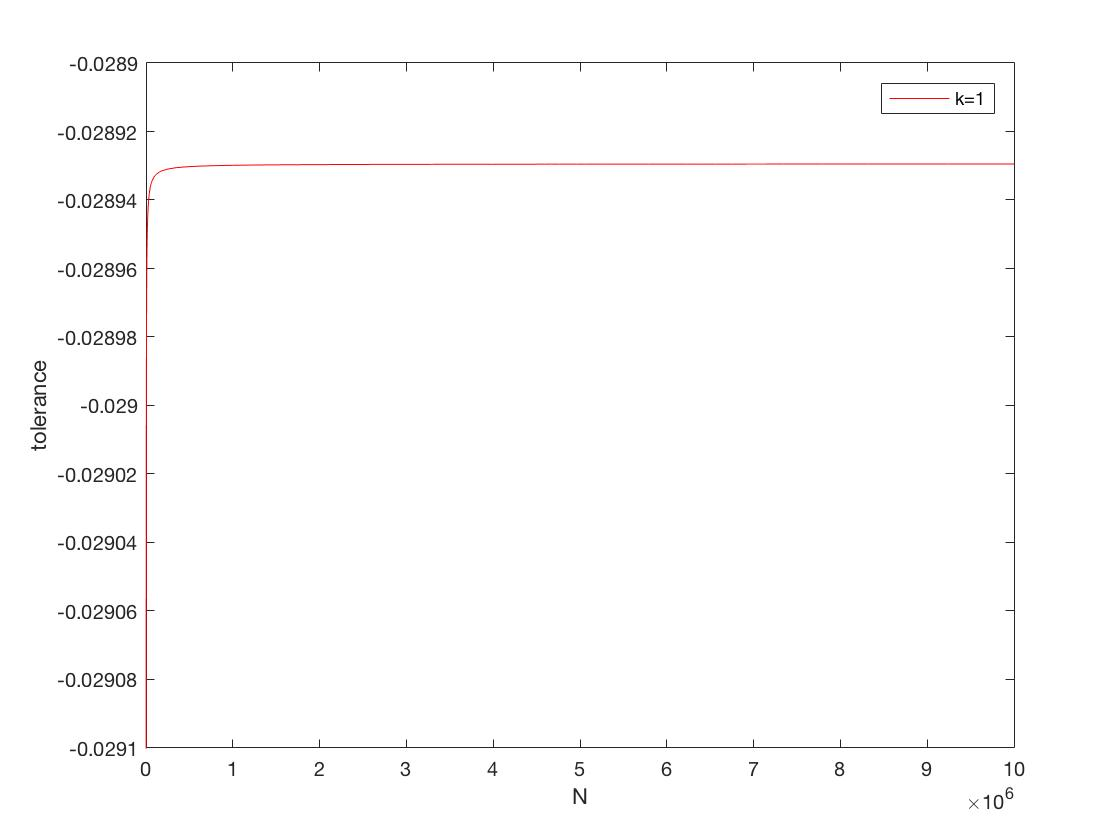
\includegraphics[width=8.8cm]{k1}}
\subfigure
{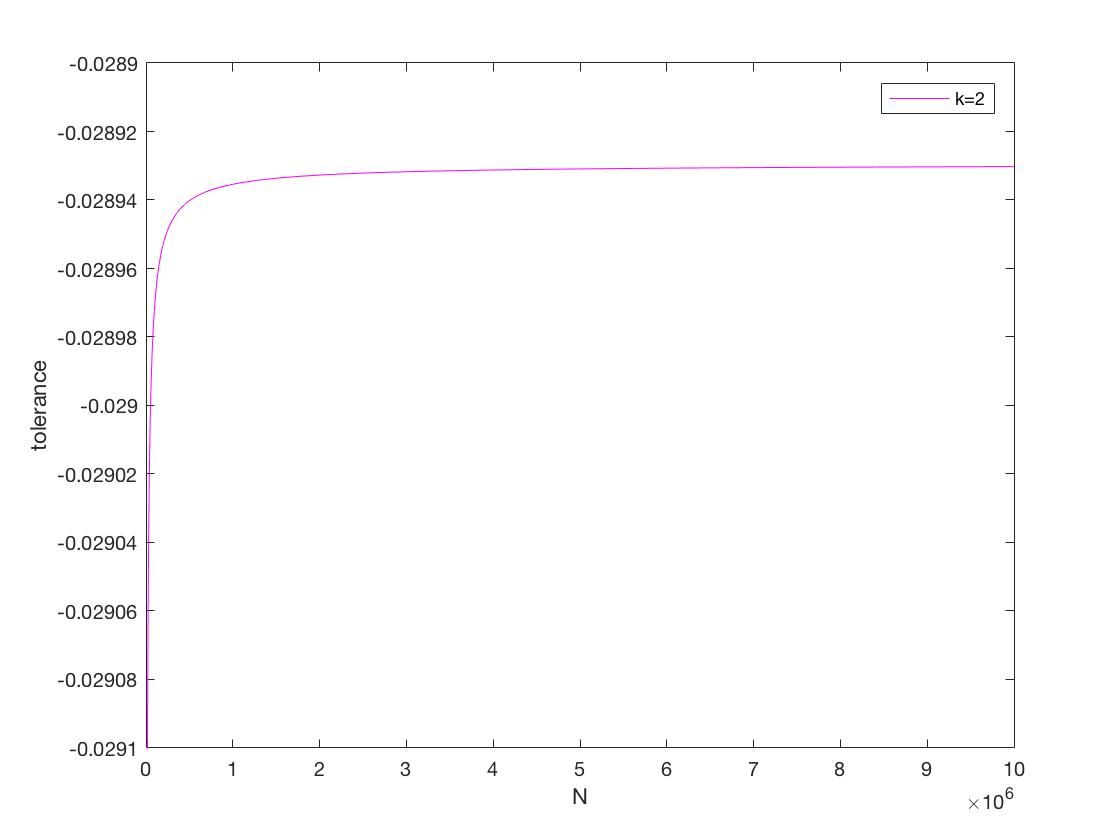
\includegraphics[width=8.8cm]{k2}}
\centering
\subfigure
{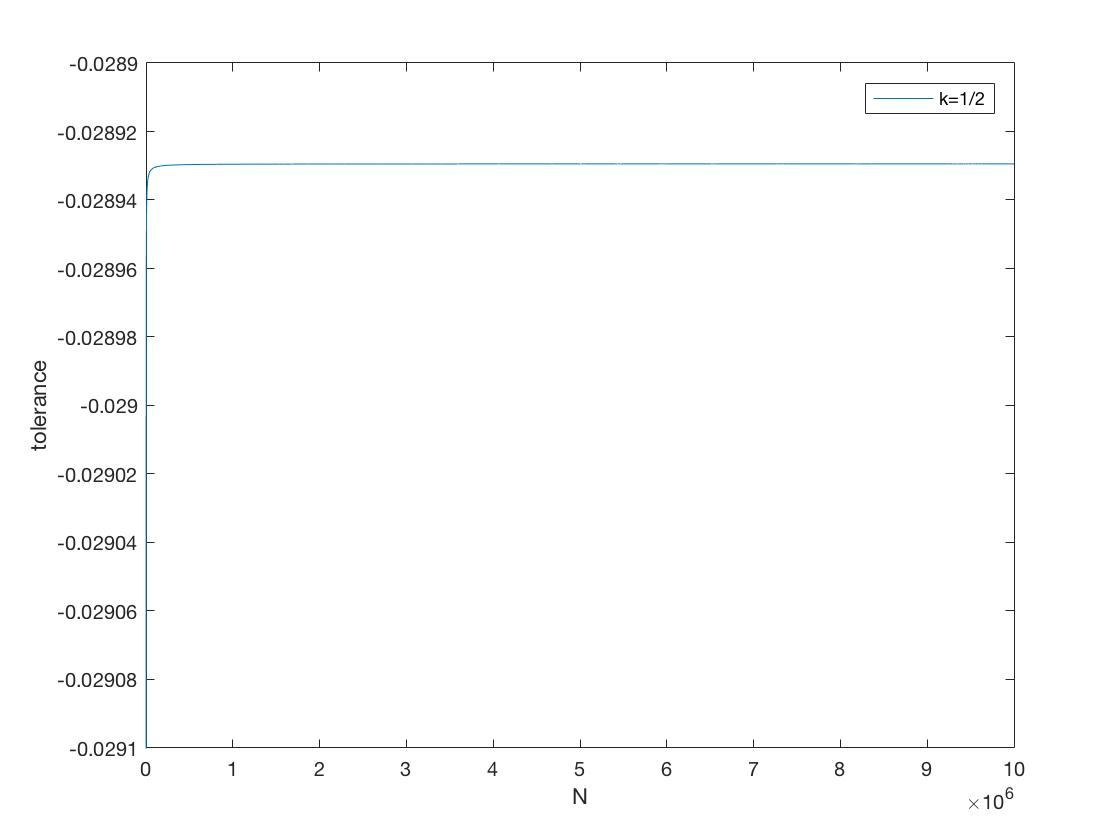
\includegraphics[width=8.8cm]{k0_5}}
\caption{Numerical estimation of the constant $C(\beta)$ for different values of $k$.}
\end{figure}